\subsection*{1.1}
    %Build a half-wave rectifier as shown below using a diode and resistor R = 33 k$\Omega$. Input
    %signal vs should be taken from the function generator. Use sinusoidal signal of frequency
    %100 Hz and amplitude about 2.5 V.

    A half-wave rectifier as shown in figure 1 below, was built using a  diode and r, R=32.5k$\Omega$ .
    A sinusoidal signal of frequency 99.96 Hz $\approx $ 100 Hz and with a amplitude 2.22 V was used as the input signal, v$_s$. The actual peak voltage is half the peak to peak voltage: $$ V_p = \dfrac{V_{p-p}}{2} = \dfrac{4.431}{2} = 2.22 \ V$$ \\

    %FIG1 CIRCUIT DIAGRAM OF A HALFWAVE RECTIFIER
    \begin{figure}[h!]
        \centering
        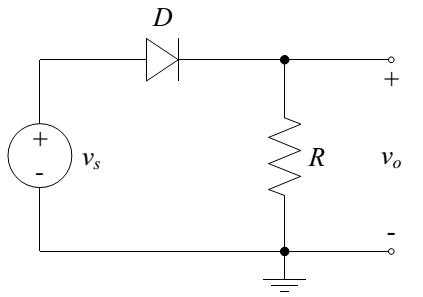
\includegraphics[width=5cm]{task1_1.png}
        \captionof{figure}{The circuit in Task 1.1}
    \end{figure}

\subsection*{1.2}
    %Observe  the  input  signal  vs and  output  signal  vo using  the  oscilloscope.  
    %Determine  the voltage drop across the diode.

    The input signal, v$_s$, and the output signal, v$_o$, were observed using the oscilloscope and the voltage drop across the diode was determined.\\

    %FIG2 OSCILLOSCOPE SHOWING INPUT AND OUTPUT SIFNALS
    \begin{figure}[h!]
        \centering
        %\includegraphics[width=5cm]{task1_2.png}
        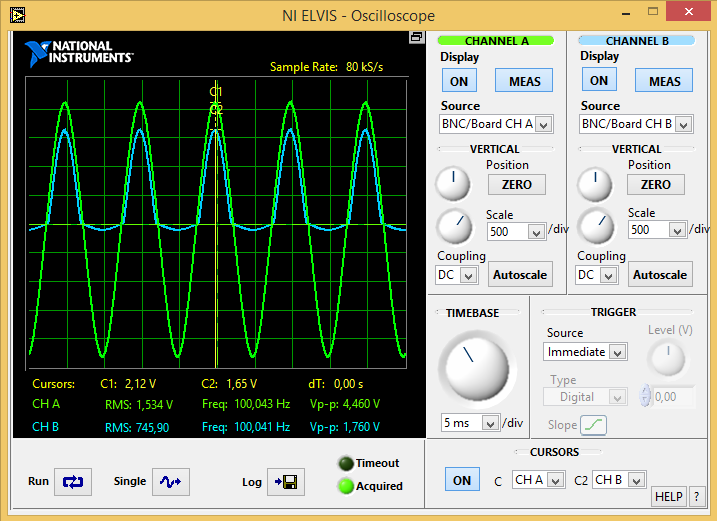
\includegraphics[width=5cm]{task1_1b.png}
        \captionof{figure}{The oscilloscope for the analysis of the circuit in figure 1}
    \end{figure}

    Using values read from the oscilloscope seen in figure 2 above, the voltage drop across the diode was determined using the following formula.

    $$V_d = V_{s,peak} - V_{o,peak} = 2.12 \ V - 1.65 \ V = 0.47 \ V$$

\subsection*{1.3}
    %Modify the rectifier circuit as shown below:

    The half-wave rectifier circuit was modified by adding a capacitor C in parallel with resistor R as shown in figure 3 below.

    %FIG3 CIRCUIT DIAGRAM OF THE MODIFIED HALF-WAVE RECTIFIER
    \begin{figure}[h!]
        \centering
        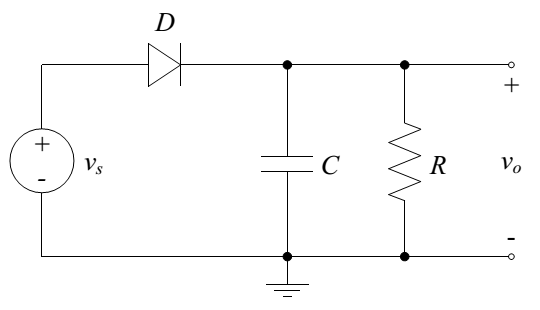
\includegraphics[width=6cm]{task1_3.png}
        \captionof{figure}{The circuit in task 1.3.}
    \end{figure}

\subsection*{1.4}
    %For each of the following capacitance values C = 0.22 µF and C = 1 µF observe the input
    %and  output  signals  using  the  oscilloscope.  Determine  the  value  of  the  ripple  voltage  in
    %each case. 
    
    The input signal, v$_s$, and the output signal, v$_o$, were observed using the oscilloscope for the following capacitance values C = 0.225 $\mu$F and C = 0.984 $\mu$F and the ripple voltage was determined.\\
    
    The theoretical value for the ripple voltage is determined with the discharging formula for a capacitor in parallel with a resistor:
    $$ V_r = V_p - V_p \ e^{-T/RC} =  V_p - V_p \ e^{-1/fRC}$$ 
    
    The peak voltage after the diode must also be recognized were that voltage is the peak voltage over the capacitor and the output:
     $$ V_p = V_{pInput} - V_d = 2.22 \ V - 0.47 \ V = 1.75 \ V$$.
    
    \begin{figure}[h!]
        \centering
        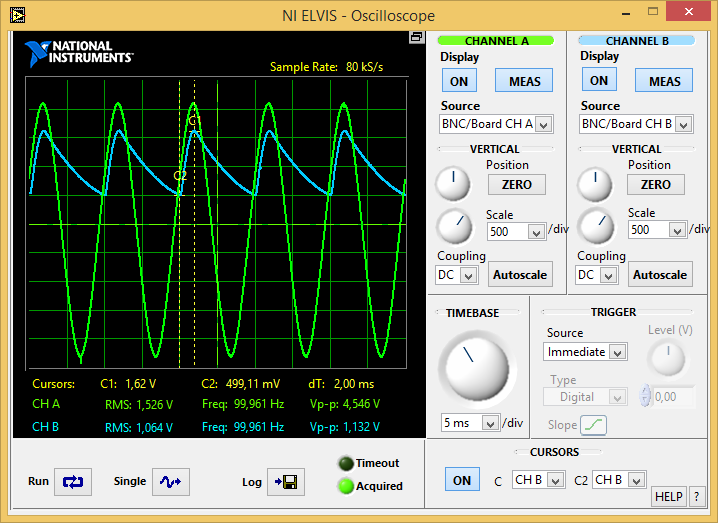
\includegraphics[width=5cm]{task1_4_022uF.png}
        \captionof{figure}{The oscilloscope for the circuit in task 1.3 with the capacitor value at $0.225 \ \mu F$ }
    \end{figure}
    
    From figure 4 the ripple voltage for the diode can be calculated from the measured data: $$ V_{r,0.225 \ \mu F} = 1.62 \ V - 0.499 \ V = 1.12 \ V $$
     The theoretical value is then calculated with the formula for a discharging capacitor:
    
     $$ V_{r,0.225 \ \mu F} = 1.75 \ V - 1.75 \ V \ e^{-1/(100 \cdot 32.5k \cdot 0.225 \ \mu F)} = 1.30 \ V $$

    \begin{figure}[h!]
        \centering
        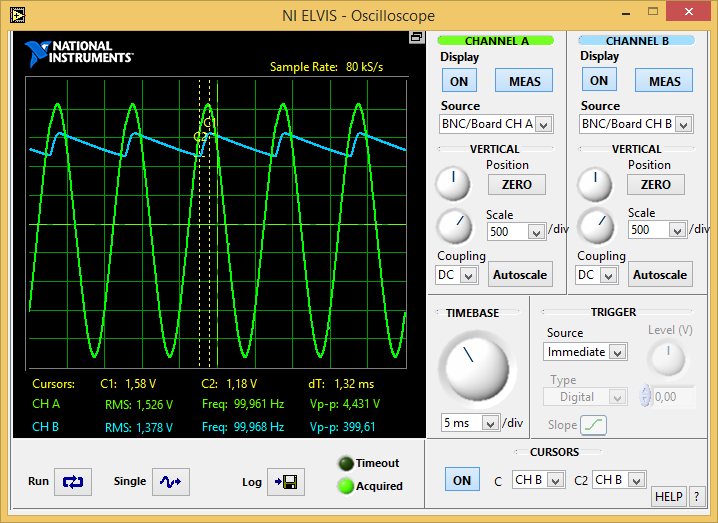
\includegraphics[width=5cm]{task1_4_1uF.png}
        \captionof{figure}{The oscilloscope for the circuit in task 1.3 with the capacitor value at $0.984 \ \mu F$ }
    \end{figure}
    
    From figure 5 the ripple voltage for the diode can be calculated from the measured data: $$V_{r,0.984 \ \mu F} = 1.58 \ V - 1.18 \ V = 0.40 \ V $$
     The theoretical value is then calculated with the formula for a discharging capacitor:
    
     $$ V_{r,0.984 \ \mu F} = 1.75 \ V - 1.75 \ V \ e^{-1/(100 \cdot 32.5k \cdot 0.984 \ \mu F)} = 0.47 \ V $$

    

\subsection*{1.5}
    %Compare  the  values  of  the  ripple  voltages  obtained  experimentally  with  the  theoretical
    %ones. 
    
       % Table generated by Excel2LaTeX from sheet 'Sheet1'
      % Table generated by Excel2LaTeX from sheet 'Sheet1'
   \begin{table}[htbp]
     \centering
     \caption{Comparison between theoretical and measured ripple voltage}
       \begin{tabular}{c|c|c|c}
       Capacitor Value [$\mu F$] & Measured ripple voltage [V] & Theoretical ripple voltage [V] & $\Delta V_r$ [V] \\
       \hline
       0.225         &     1.62 - 0.499 = 1.12        & 1.30 & 0.18 \\
       0.984         &     1.58 - 1.18 = 0.40         & 0.47 & 0.07 \\       
       \end{tabular}%
     \label{tab:addlabel}%
   \end{table}%

The theoretical values and the measured values match very well and the error is not significant.

    



